\begin{center}
\fbox{\fbox{\parbox{6.5in}{\centering
\begin{flushleft}

\vspace{2mm}
\hspace{5mm}
\textbf{\underline{Kolmnurga välisnurk}}

\vspace{2mm}
\hspace{5mm}
Meenutame, et kolmnurga sisenurkade summa on $180^{o}$. Ehk joonise alusel $\boxed{\alpha + \beta + \gamma = 180^{o}}$.


\begin{center}
\begin{tikzpicture}[scale=0.5]

\coordinate (A) at (0,0);
\coordinate (B) at (-2,-4);
\coordinate (C) at (9,-4);

\draw[line width=0.3mm, blue]  (A) to (B) to (C) to (A);
\node[below] at (0.2,-0.25){$\alpha$};
\node[right] at (-1.75,-3.5){$\beta$};
\node[left] at (7.95,-3.7){$\gamma$};

\pic [draw, angle radius= 0.5cm] {angle=B--A--C};
\pic [draw, angle radius=7mm] {angle=C--B--A};
\pic [draw, angle radius= 10mm] {angle=A--C--B};
\end{tikzpicture}
\end{center}

\hspace{5mm}
NB! Kolmnurga sisenurkade summa ei sõltu kolmnurga kujust! Ükskõik millise kolmnurga sisenurkade\\ \hspace{5mm} summa on alati $180^{o}.$

\vspace{2mm}
\hspace{5mm}
\textbf{\underline{Välisnurk}}

\vspace{2mm}
\hspace{5mm}
Kui pikkendada ühte kolmnurga külge tippust, siis tekkib tema sisenurga kõrvale välisnurk.

\begin{center}
\begin{tikzpicture}[scale=0.5]

\coordinate (A) at (0,0);
\coordinate (B) at (-2,-4);
\coordinate (C) at (9,-4);
\coordinate (D) at (13,-4);
\coordinate (E) at (13.5,-6);

\draw[line width=0.3mm, blue]  (A) to (B) to (C) to (A);
\node[below] at (0.2,-0.25){$\alpha$};
\node[right] at (-1.75,-3.5){$\beta$};
\node[left] at (7.95,-3.7){$\gamma$};

\draw[line width=0.2mm, black] (C) to (D);
\draw[line width=0.2mm, black, dashed] (C) to  (E);

\pic [draw, angle radius= 0.5cm] {angle=B--A--C};
\pic [draw, angle radius=7mm] {angle=C--B--A};
\pic [draw, angle radius= 10mm] {angle=A--C--B};

\node at (9.1,-3.6){$\delta$};
\pic [draw, angle radius= 5mm] {angle = D--C--A};

\node at(10.75,-4.4) {$\gamma$};
\pic [draw, angle radius = 12.5mm] {angle=E--C--D};
\pic [draw, angle radius= 6mm]{angle=B--C--E};
\node at (8.9,-4.4){$\delta$};
\end{tikzpicture}
\end{center}

\hspace{5mm}
Joonisel on välisnurgaks nurk $\delta$. On näha, et pikkendatud külg moodustab sirgnurga. Kuna sirgnurga\\ \hspace{5mm} väärtus on $180^{o}$, siis peaks olema loomulik, et kolmnurga sisenurga ja välisnurga summa peaks samuti\\ \hspace{5mm} andma meile $180^{o}$. Ehk:

\begin{equation}
\label{30_eq1}
\boxed{\delta + \gamma = 180^{o}}
\end{equation}

\hspace{5mm}
Kui avaldada valemist välisnurk $\delta$, siis saame:

\begin{equation}
\label{30_eq2}
\boxed{\delta=180^{o}-\gamma}
\end{equation}

\vspace{5mm}
\hspace{5mm}
\textbf{\underline{Kolmnurga mediaanid}}

\vspace{2mm}
\hspace{5mm}
Kolmnurga mediaan on lõik, mis ühendab kolmnurga tippu ja tema vastaskülje keskpunkti. Iga\\ \hspace{5mm} mediaan jaotab kolmnurga kaheks kolmnurgaks, \textbf{mille pindalad on võrdsed.}

\begin{center}
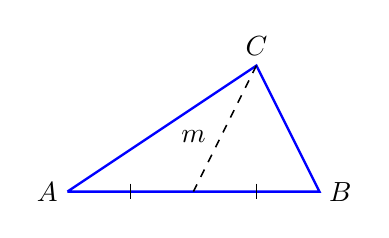
\begin{tikzpicture}[scale=0.4]

\coordinate (A) at (0,0);
\coordinate (B) at (8,0);
\coordinate (C) at (6,4);
\coordinate (D) at (4,0);

\draw[line width=0.3mm, blue] (A) to (B) to (C) to (A);
\draw[line width=0.2mm, black, dashed] (C) to (D);
\draw[line width=0.2mm, black ] (2,0.25) to (2,-0.25);
\draw[line width=0.2mm, black] (6, 0.25) to (6, -0.25);

\node[left] at (A){$A$};
\node[right] at (B){$B$};
\node[above] at (C){$C$};
\node at (4,1.75){$m$};

\end{tikzpicture}
\end{center}

\hspace{5mm}
\textbf{Teoreem:} Kolmnurga kõik mediaanid lõikuvad ühes punktis, mis jaotab iga mediaani suhtes 2:1.\\ \hspace{5mm}Ehk mediaani tipupoolne osa on 2 korda pikkem, kui küljepoolne osa.

\end{flushleft}
}}}
\end{center}


\pagebreak

\begin{center}
\fbox{\fbox{\parbox{6.5in}{\centering
\begin{flushleft}

\vspace{5mm}
\hspace{5mm}
Mediaanide lõikepunktil on üks märkimisväärne omadus. Nimelt asub kolmnurga mediaanide\\ \hspace{5mm} lõikepunktis kolmnurga raskuskese, mis tähendab, et selles punktis on kolmnurk tasakaalus.

\begin{center}
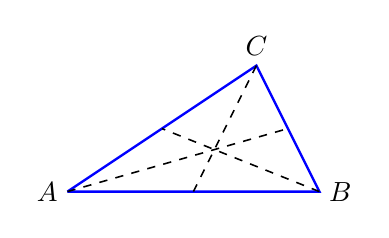
\begin{tikzpicture}[scale=0.4]

\coordinate (A) at (0,0);
\coordinate (B) at (8,0);
\coordinate (C) at (6,4);
\coordinate (m1) at (4,0);

\draw[line width=0.3mm, blue] (A) to (B) to (C) to (A);
\draw[line width=0.2mm, black, dashed] (C) to (m1);

\path (B)--(C) coordinate[pos=0.5](m2);
\path (C)--(A) coordinate[pos=0.5](m3);

\draw[line width=0.2mm, black, dashed] (A) to (m2);
\draw[line width=0.2mm, black, dashed] (B) to (m3);

\node[left] at (A){$A$};
\node[right] at (B){$B$};
\node[above] at (C){$C$};

\end{tikzpicture}
\end{center}


\end{flushleft}
}}}
\end{center}


\vspace{0.5cm}

\textbf{Märkmed}\\
\vspace{2mm}
\begin{mdframed}[style=graphpaper]
\vspace{15cm}
\end{mdframed}